\documentclass{beamer}

\usetheme{metropolis}

\usepackage{algorithm,algorithmic}

\title{Minimisation de machines de Turing, application au problème 2Color}
\date{\today}
\author{Elowan Harnisch}
\begin{document}
    \maketitle
    \begin{frame}{Machine de Turing}
        \begin{alert}{Définition}
            Une machine de Turing est un sixtuplet $(Q, \Sigma, S, q_0, F, \delta)$ où:
            \begin{itemize}
                \item $Q$ est un ensemble fini d'états
                \item $\Sigma$ est un ensemble fini de symboles
                \item $S \notin \Sigma$ est le symbole blanc
                \item $q_0 \in Q$ est l'état initial
                \item $F \subseteq Q$ est l'ensemble des états acceptants
                \item $\delta: Q \times \Sigma \rightarrow Q \times \Sigma \times \{L, R\}$ est la fonction de 
                transition
            \end{itemize}
            Elle possède de plus une bande infinie sur laquelle elle peut
            lire et écrire les symboles de $\Sigma \cup {S}$.
        \end{alert}
    \end{frame}
    \begin{frame}{Machine de Turing}
        \begin{figure}[t]
            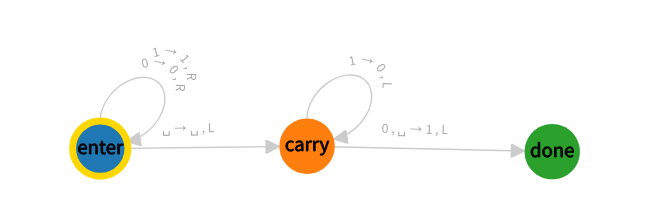
\includegraphics[width=0.8\textwidth]{images/MT.png}
            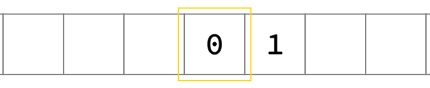
\includegraphics[width=0.4\textwidth]{images/bande1.png}
            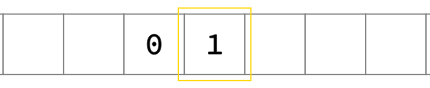
\includegraphics[width=0.4\textwidth]{images/bande2.png}
            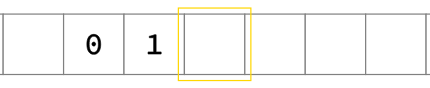
\includegraphics[width=0.4\textwidth]{images/bande3.png}
            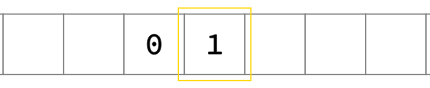
\includegraphics[width=0.4\textwidth]{images/bande4.png}
            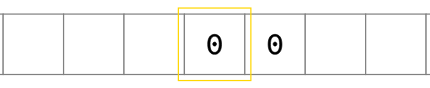
\includegraphics[width=0.4\textwidth]{images/bande5.png}
            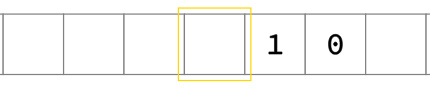
\includegraphics[width=0.4\textwidth]{images/bande6.png}
            \caption{Schema d'execution de machine de Turing qui ajoute 1 à un 
            nombre binaire}
        \end{figure}
    \end{frame}
    \begin{frame}{Automate fini déterministe (DFA)}
        \begin{alert}{Définition}
            Un automate fini déterministe (DFA) est un quintuplet 
            $(Q, \Sigma, q_0, F, \delta)$ où:
            \begin{itemize}
                \item $Q$ est un ensemble fini d'états
                \item $\Sigma$ est un ensemble fini de symboles
                \item $q_0 \in Q$ est l'état initial
                \item $F \subseteq Q$ est l'ensemble des états finaux
                \item $\delta: Q \times \Sigma \rightarrow Q$ est la 
                fonction de transition
            \end{itemize}
        \end{alert}
    \end{frame}
    \begin{frame}{Automate fini déterministe (DFA)}
        \begin{figure}[t]
            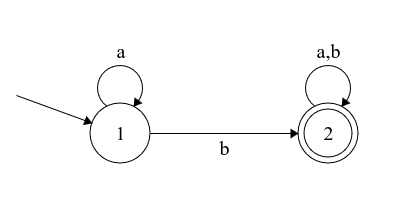
\includegraphics[width=0.9\textwidth]{images/automaton.png}
            \caption{Schema d'un automate reconnaissant le langage des mots ayant au 
            moins un b}
        \end{figure}
    \end{frame}
    \begin{frame}{Minimisation d'un DFA}
        \begin{alert}{Définition}
            La minimisation d'un automate fini déterministe est le processus 
            qui consiste à réduire le nombre d'états de l'automate tout en 
            conservant le langage reconnu. 
        \end{alert}
        \begin{block}{Théorème}
            L'algorithme de Hopcroft permet depuis un automate fini déterministe 
            d'obtenir un automate minimal reconnaissant le même langage.
        \end{block}
    \end{frame}
    \begin{frame}{Minimisation d'un automate fini déterministe}
            \begin{algorithm}[H]
                \tiny
                \algsetup{linenosize=\tiny}
                \caption{Algorithme de Hopcroft, $A = (Q, \Sigma, q_0, F, \delta)$ un automate fini déterministe}
                \begin{algorithmic}[1]
                    \STATE $P \gets \{F, Q \setminus F\}$
                    \STATE $W \gets \{\}$
                    \FOR{for $a \in \Sigma$ do}
                        \STATE ajouter $(min(F, Q \setminus F), a)$ à $W$
                    \ENDFOR
                    \WHILE{$W \neq \{\}$ do}
                        \STATE retirer $(Z, a)$ de $W$
                        \FOR{$X \in P$ tel que $X$ est coupé par $(Z, a)$ en $X'$ et $X''$ do}
                            \STATE remplacer $X$ par $X'$ et $X''$ dans $P$
                            \FOR{$b \in \Sigma$ do}
                                \IF{$(X, b)$ est dans $W$}
                                    \STATE remplacer $(X, b)$ par $(X', b)$ et $(X'', b)$ dans $W$
                                \ELSE
                                    \STATE ajouter  $min((X', b),(X'', b))$ à $W$
                                \ENDIF
                            \ENDFOR
                        \ENDFOR
                    \ENDWHILE
                \end{algorithmic}
            \end{algorithm}
    \end{frame}
    \begin{frame}{Minimisation d'une machine de Turing}
        \begin{alert}{Transformation d'une machine de Turing en DFA}
            Soit une machine de Turing $M = (Q, \Sigma, S, q_0, F, \delta)$, on
            peut construire un DFA $A = (Q, \Sigma', q_0, F, \delta')$ tel que:
            \begin{itemize}
                \item $\Sigma' = \Sigma \cup \{aKb | ((a,b)\in\Sigma^2, K\in\{R,L\})\} \cup \{S\}$
                \item $\delta'(q, aKb) = q'$, avec $(q', b, K) = \delta(q, a)$ et $a \in \Sigma, q \in Q$

            \end{itemize}
            On appelle $f$ la fonction qui réalise cette transformation.

            On en déduit son inverse en décomposant chaque lettre de A
        \end{alert}
        \begin{block}{Théorème}
            La composition de $f$, de l'algorithme de minimisation de Hopcroft 
            et de $f^{-1}$ permet d'obtenir une machine de Turing de taille au plus égale à celle de
            départ.
        \end{block}
    \end{frame}
    \begin{frame}{Problème n-2Color}
        \begin{alert}{Définition}
            Le problème 2Color est un problème de décision qui consiste à déterminer 
            si un graphe est coloriable avec 2 couleurs. 
        \end{alert}
        \begin{block}{Théorème}
            Le problème 2Color est décidable.
        \end{block}
        \begin{alert}{Définition}
            Le problème n-2Color est un problème de décision qui consiste à déterminer 
            si un graphe est coloriable avec 2 couleurs pour un graphe de maximum n sommets.
        \end{alert}
        \begin{block}{Théorème}
            Le problème n-2Color est décidable.
        \end{block}
    \end{frame}
    \begin{frame}{Problème n-2Color}
        \begin{figure}
            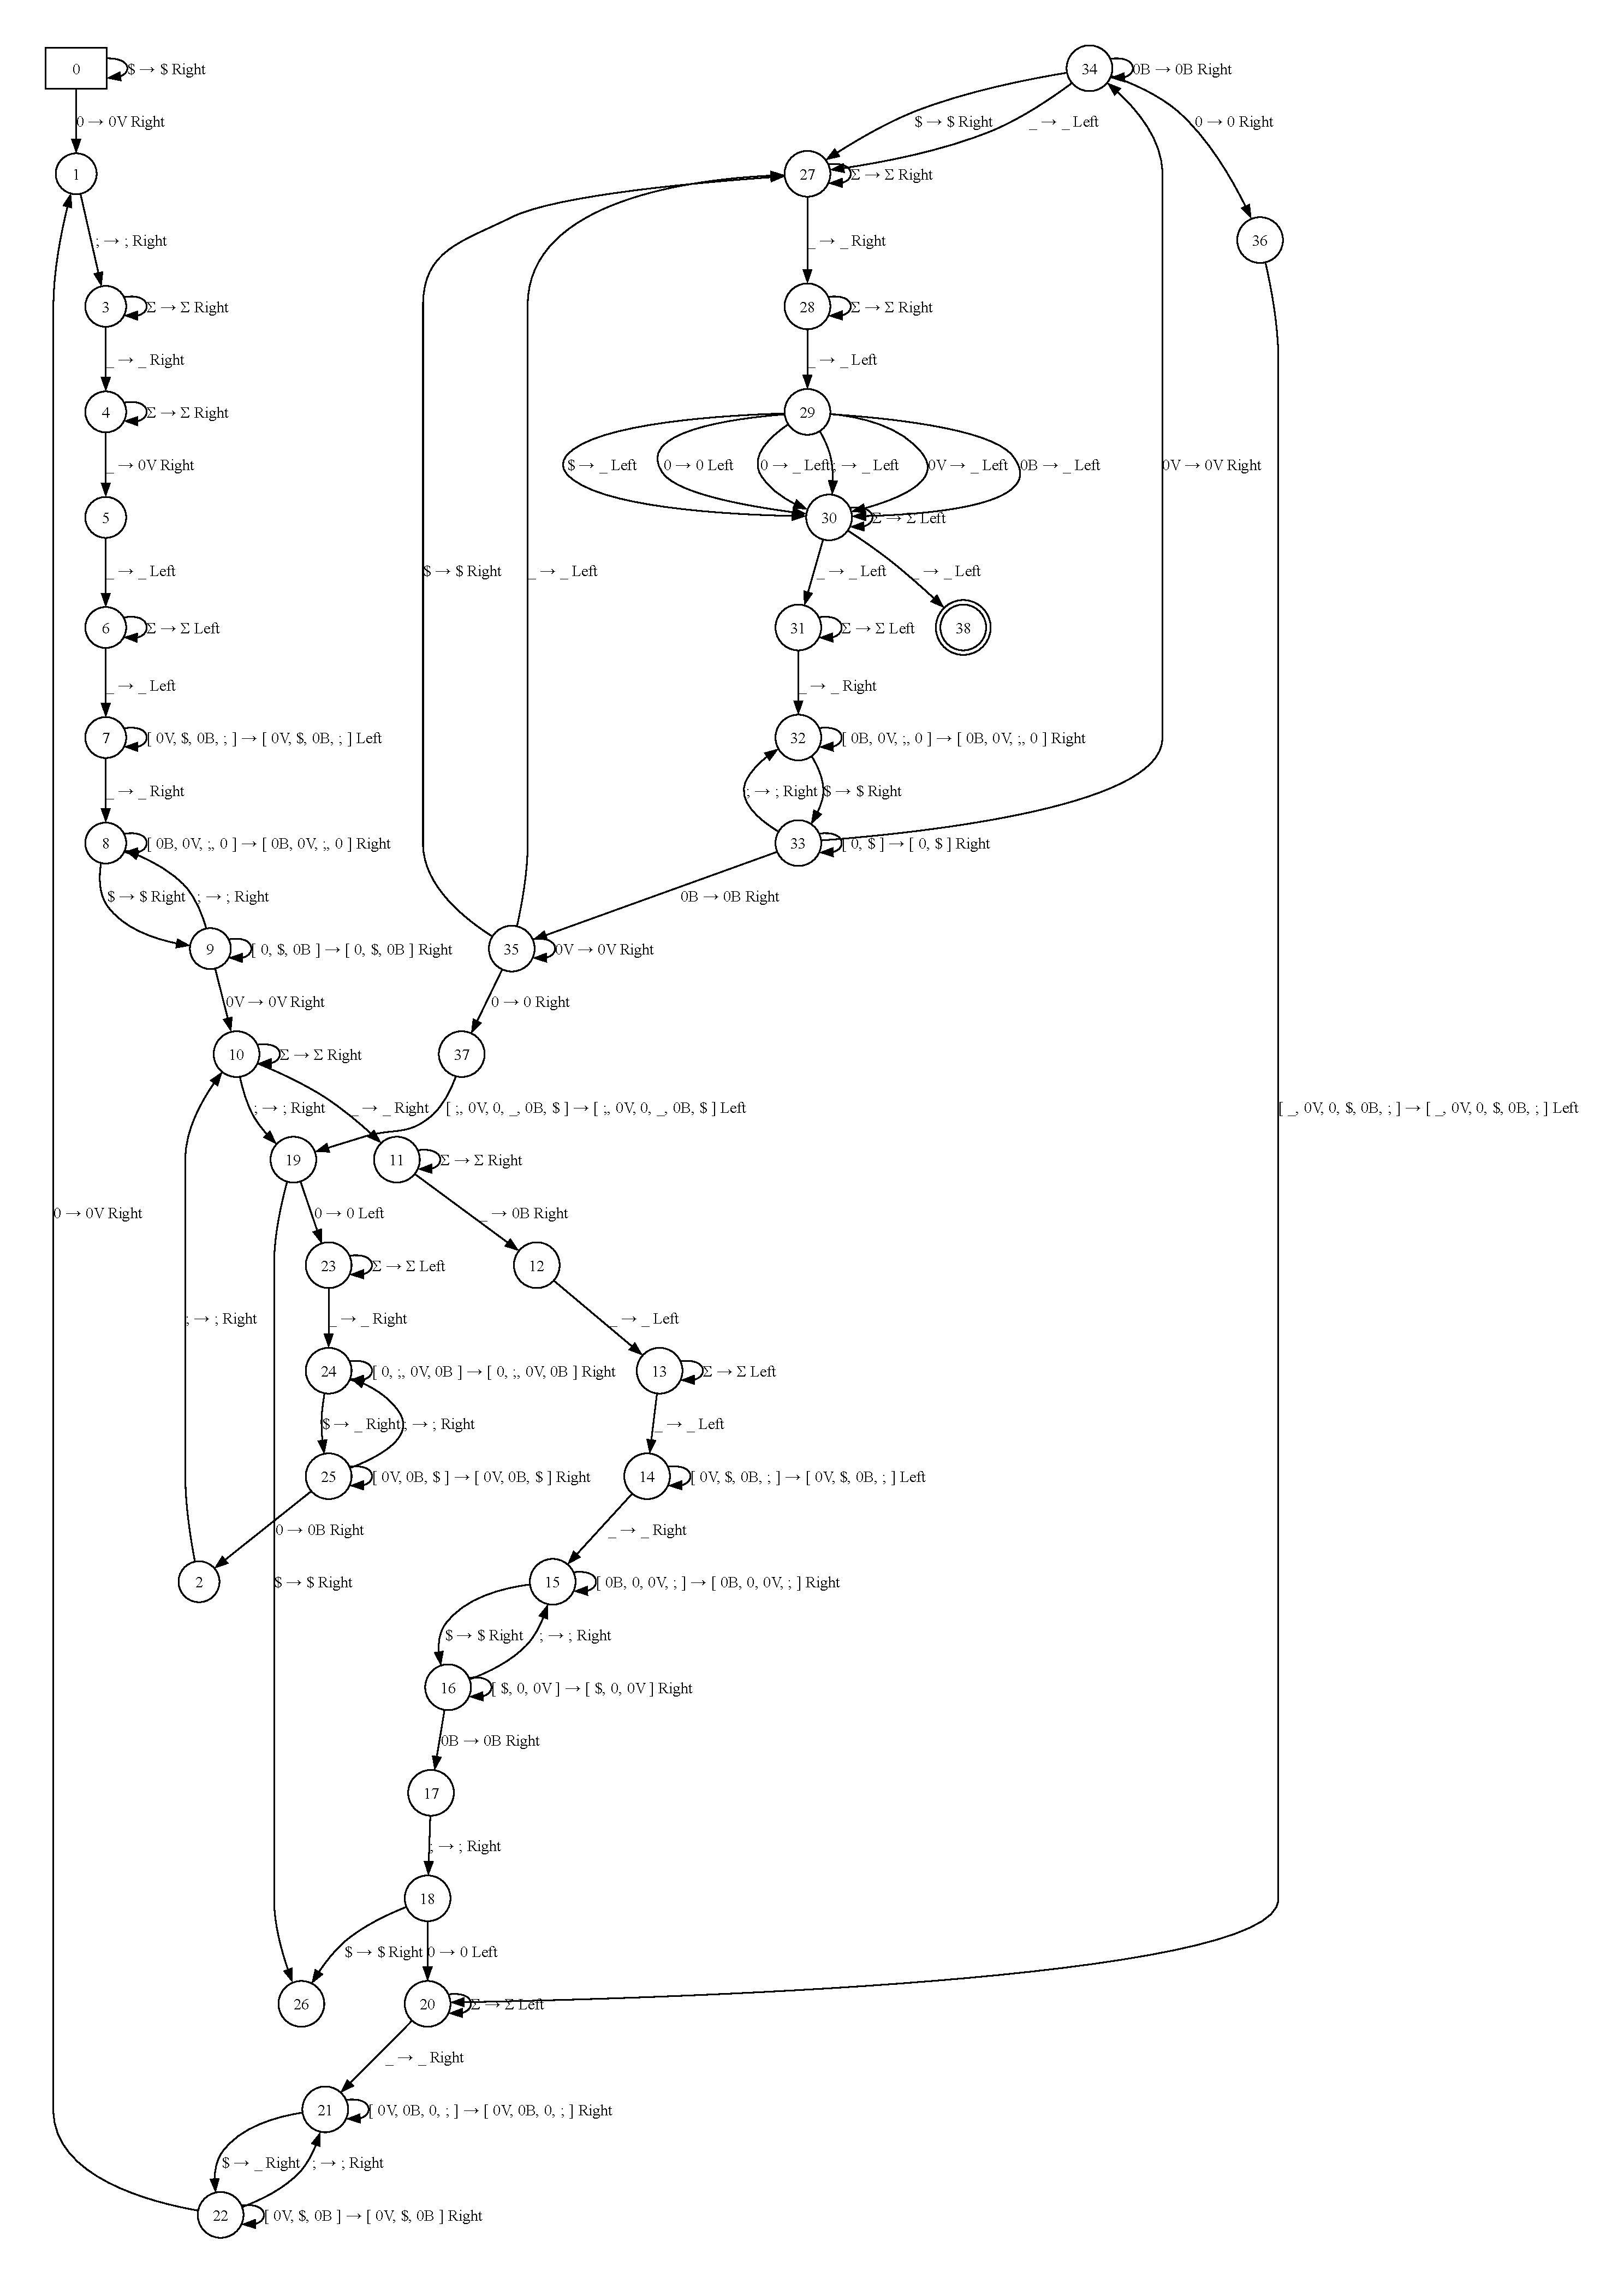
\includegraphics[width=0.4\textwidth]{images/MT_2Color_2.pdf}
            \caption{Machine de Turing créée pour résoudre le problème 2Color,
            pour un graphe de 2 sommets maximum}
        \end{figure}
    \end{frame}
    \begin{frame}{Conclusion}
        Pour la suite j'aimerais :
        \begin{itemize}
            \item Bien comprendre la preuve de l'algorithme de Hopcroft et mieux 
            l'adapter aux machines de Turing plutôt que mon bricolage actuel (même 
            si je pense que ce n'est pas possible, dans ce cas démontrer que ce problème
            n'est pas décidable mais qu'on peut essayer de s'en approcher par cette méthode)
            \item Finir de débugger la machine de Turing pour le problème n-2Color 
        \end{itemize}
    \end{frame}
\end{document}